\documentclass{alex_hü}

\name{Alexander Helbok}
\course{PS Physik}
\hwnumber{2}


\begin{document}
\renewcommand{\labelenumi}{\alph{enumi}.}


\begin{mybox}{1. Influenz in einer Metallplatte}
	\centering \( k = \tfrac{1}{4\pi \epsilon_0};\quad r^2 = x^2+y^2;\quad  \sigma = \epsilon_0 E \)
	\tcblower
		\begin{flalign*}
			E_1(x,y,z) &= k\tfrac{Q}{x^2+y^2+(z+R)^2} &&\\
			E_2(x,y,z) &= E_1(x,y,z-2R) = k\tfrac{Q}{x^2+y^2+(z-R)^2} &&\\
			E_{ges}(x,y,z) &= E_1 + E_2 = kQ\left( \tfrac{1}{x^2+y^2+(z+R)^2} + \tfrac{1}{x^2+y^2+(z-R)^2} \right) &&\\[2ex]
			\sigma(r) &= \epsilon_0 E_{ges}(x,y,z) = \epsilon_0kQ\left( \tfrac{1}{x^2+y^2+(z+R)^2} + \tfrac{1}{x^2+y^2+(z-R)^2} \right) &&\\
			&=\dl{\tfrac{Q}{2\pi}\tfrac{1}{r^2+R^2}} &&
		\end{flalign*}
\end{mybox}


\begin{mybox}{2. Feld einer Hohlkugel}
	\centering \( k = \tfrac{1}{4\pi \epsilon_0} \)
	\tcblower
	\begin{enumerate}
		\item \( \rho = \tfrac{Q}{V} \)
		\begin{flalign*}
			V &= \int_V dV = \int\limits_{0}^{\pi}\int\limits_{0}^{2\pi}\int\limits_{R_i}^{R_a} r^2\sin(\theta)\ \mathrm{d}r\mathrm{d}\varphi\mathrm{d}\theta &&\\
			&= \tfrac{4}{3}\pi(R_a^3-R_i^3) &&\\
			\rho &= \dl{\tfrac{3Q}{4\pi} \tfrac{1}{R_a^3-R_i^3}} &&\\
		\end{flalign*}
		For  \(r \geq R_a\):
		\begin{flalign*}
			\hspace{3cm} q_{in} &= Q &&\\
			\frac{q_{in}}{\epsilon_0} &= \oint \vec{E}(\vec{r})\ \mathrm{d}\vec{A} = E(r) \oint \mathrm{d}A = E(r)4\pi r^2 &&\\
			E(r) &= kQ \tfrac{1}{r^2} &&
		\end{flalign*}
		For \(R_i < r < R_a\):
		\begin{flalign*}
			\hspace{3cm} q_{in} &= \rho V_{in} = Q \tfrac{r^3-R_i^3}{R_a^3-R_i^3} &&\\
			\tfrac{q_{in}}{\epsilon_0} &= \oint \vec{E}(\vec{r})\ \mathrm{d}\vec{A} = E(r) \oint \mathrm{d}A = E(r)4\pi r^2 &&\\
			E(r) &= kQ \tfrac{r^3-R_i^3}{R_a^3-R_i^3}\tfrac{1}{r^2} &&
		\end{flalign*}
		For \( r \leq R_i\):
		\begin{flalign*}
			\hspace{3cm} q_{in} &= 0 &&\\
			E(r) &= 0 &&
		\end{flalign*}
		\boxed{
		\begin{aligned}
			E(r) = \begin{cases}
				0& \quad $for $\ 0 < r \le R_i, \\
				\tfrac{kQ}{R_a^3-R_i^3} \left(r - \tfrac{R_i^3}{r^2}\right)& \quad $for $\ R_i < r < R_a, \\
				kQ \tfrac{1}{r^2}& \quad $for $\ R_a \le r. 
			\end{cases} 
		\end{aligned}
		}
	\tcbline
		\begin{minipage}{\textwidth}
			\hspace{1cm}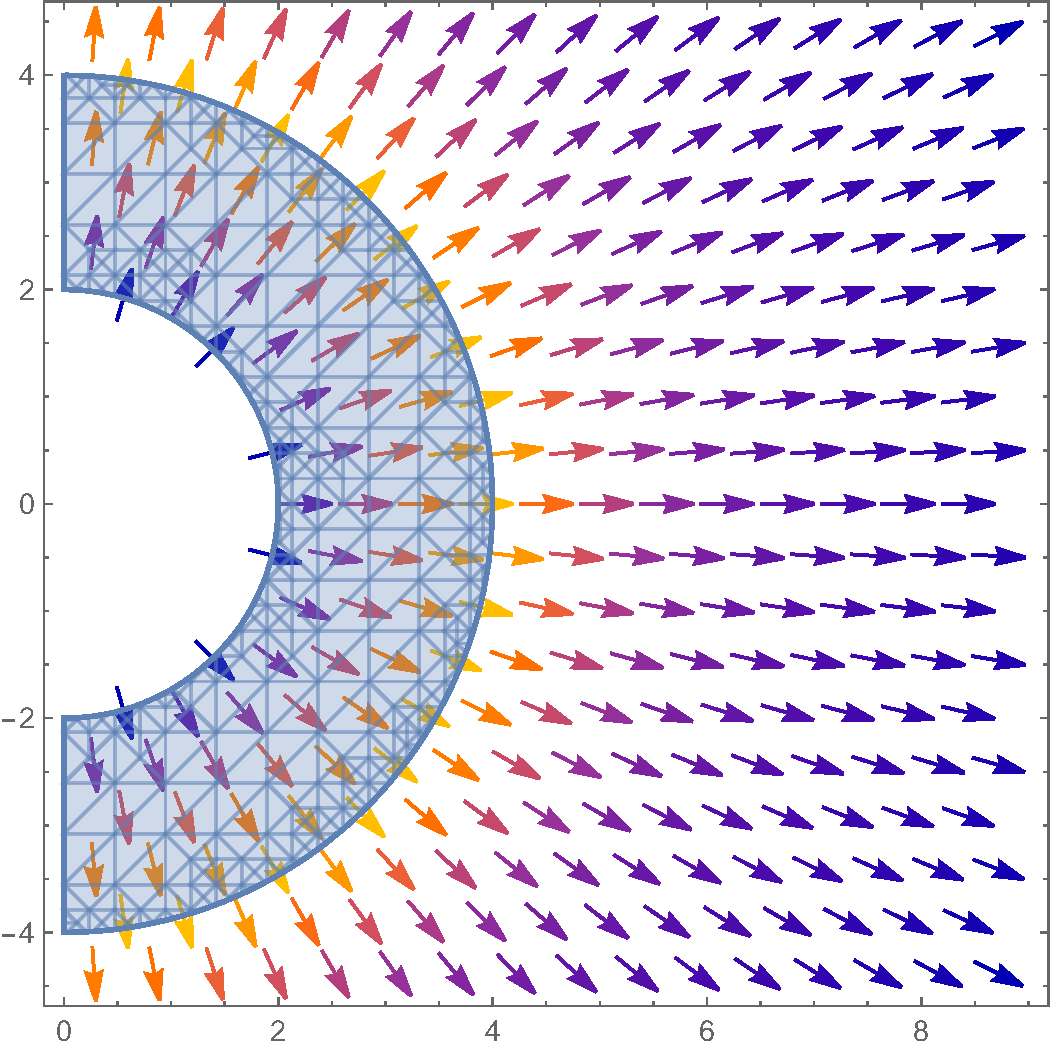
\includegraphics[width=0.5\textwidth]{1.pdf}
			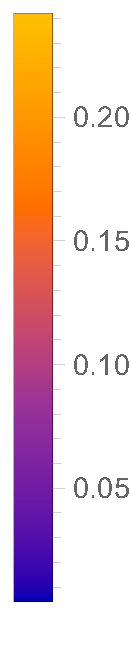
\includegraphics[scale=0.7]{2.pdf}
		\end{minipage}\vspace{0.5cm}
		\begin{tikzpicture}
			\begin{axis}[
				width=250pt,
				height=150pt,
				axis lines=center,
				%y axis line style={thick},
				tick align=outside,
				xmin=0,xmax=10,ymin=0,ymax=0.35,
				xlabel style={below},
				xtick = {2,4}, ytick = {0.25},
				xticklabels={\( R_i \), \( R_a \)},
				yticklabels={\( E_{max} \)},
				xlabel=$r$,
				ylabel=$E$,
				grid=major,
				grid style={thin,densely dotted,black!20},
				%legend columns=2,
				legend style={at={(axis description cs:1,0.35)},anchor=east}]
				\addplot [-, thick,  blue, domain = 4:10, smooth] {1/(x-2)^2};
				\addplot [-, thick,  blue, domain = 2:4, smooth] {(x-2)/(4-2)^3};
				\draw[blue, thick] (0,0) -- (2,0);
			\end{axis}
		\end{tikzpicture}\\
		\begin{minipage}{\textwidth}
			\vspace{-1cm}\hspace{0.4cm}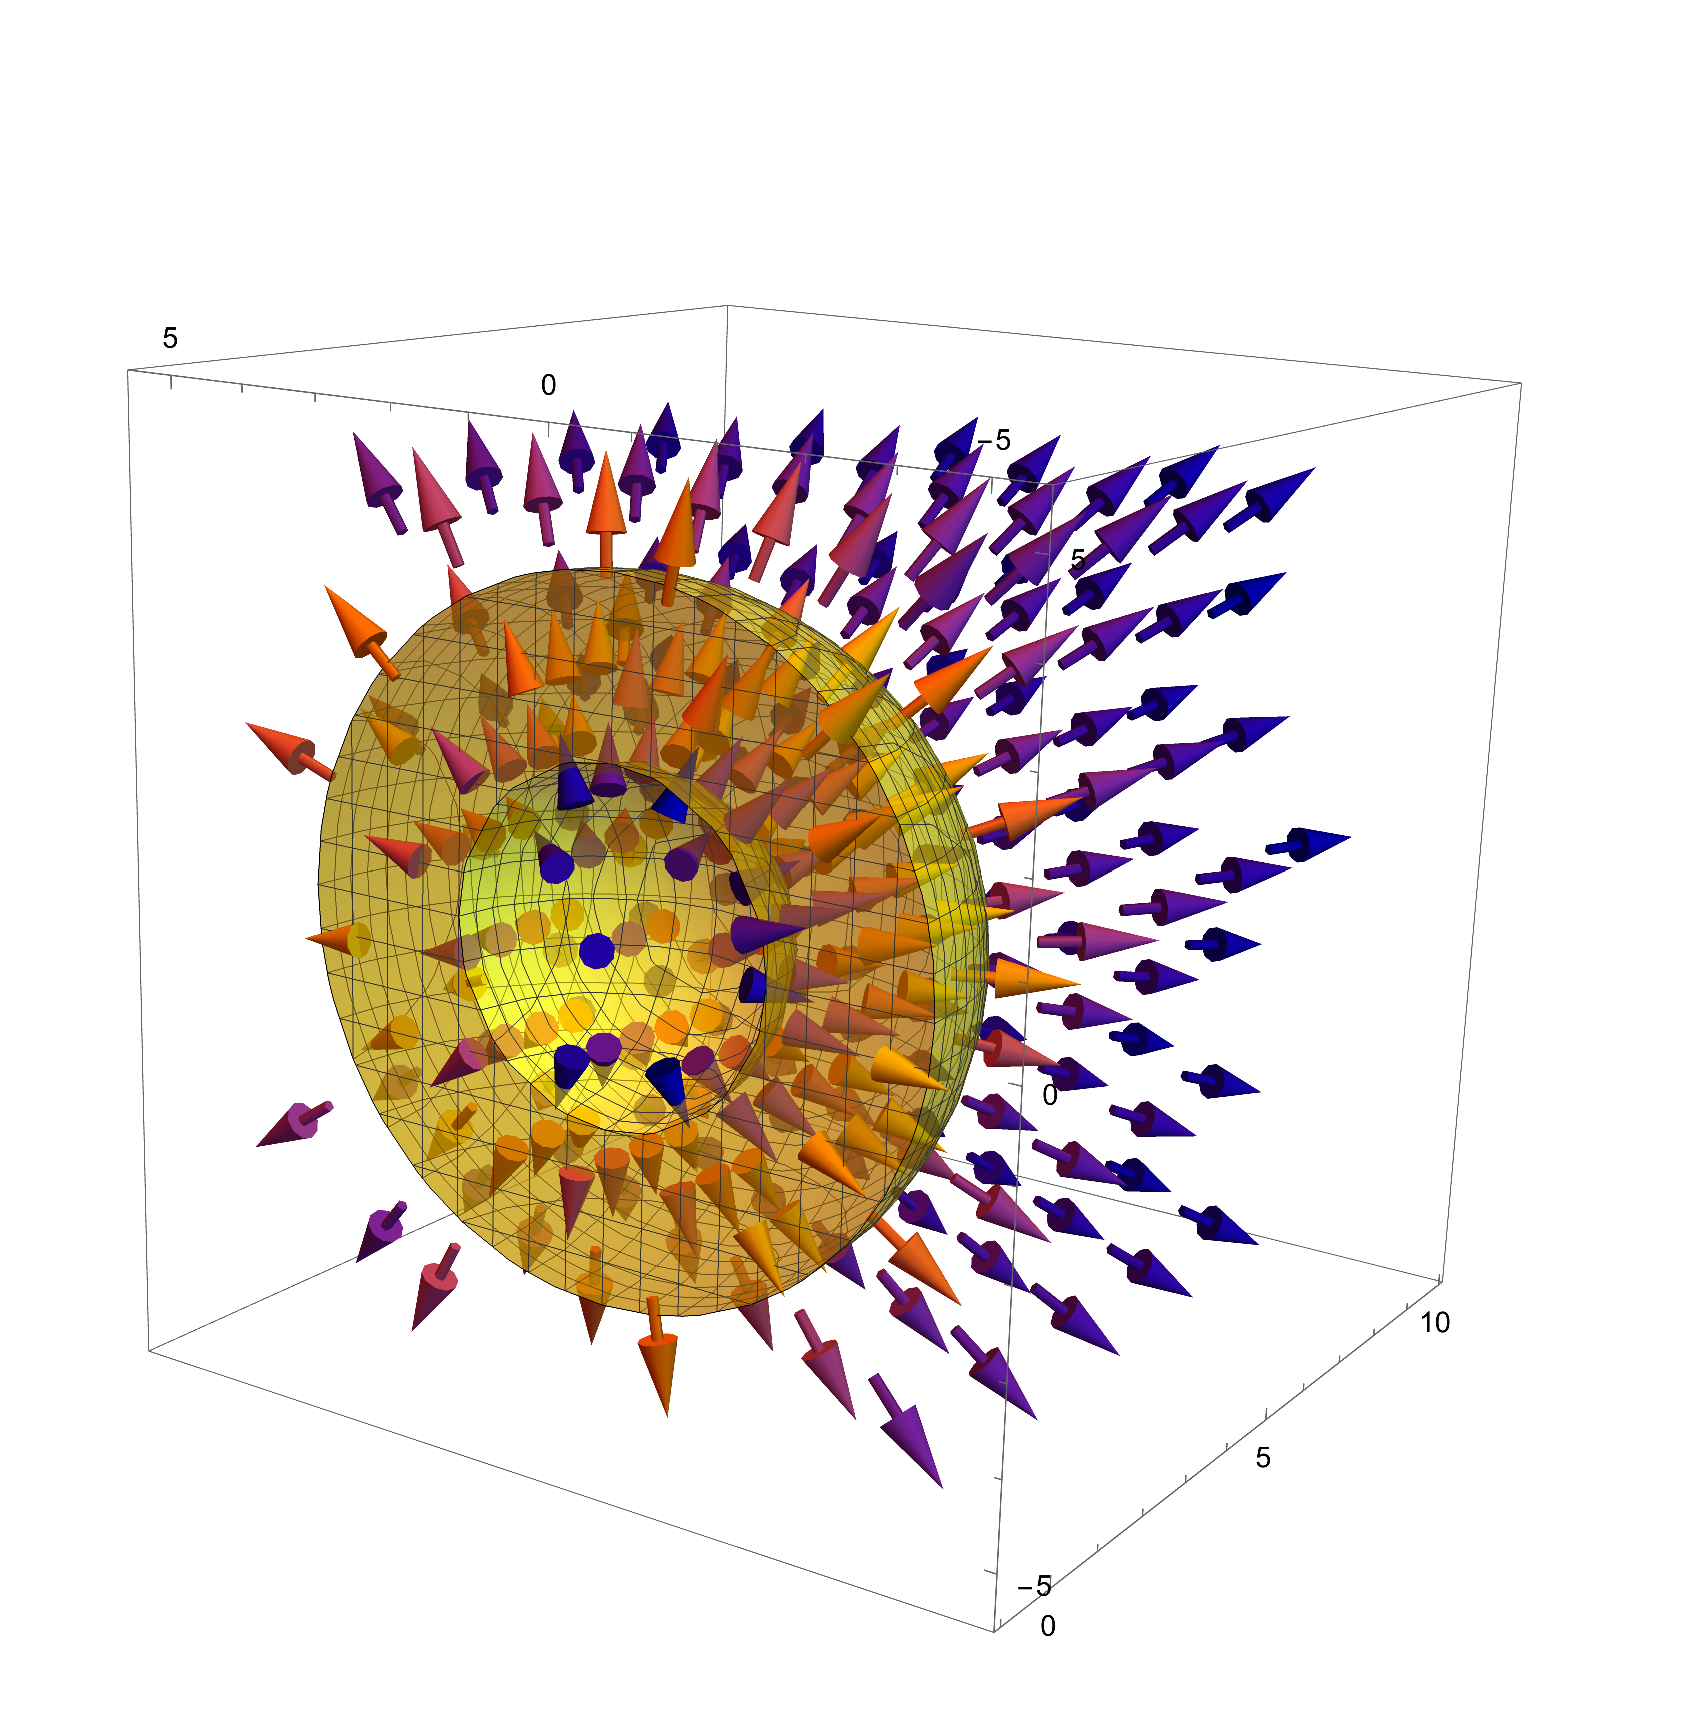
\includegraphics[width=0.65\textwidth]{3.pdf}
			\hspace{-0.6cm}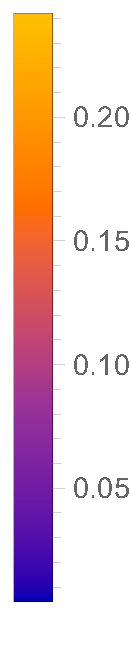
\includegraphics[scale=0.77]{2.pdf}
		\end{minipage}
	\end{enumerate}
\end{mybox}


\begin{mybox}{3. Zwei ringförmige Ladungsträger}
	\centering \( k = \tfrac{1}{4\pi \epsilon_0} \)
	\tcblower
	\begin{enumerate}
		\item \(h = \sqrt{r^2+z^2};\quad \cos(\theta) = \tfrac{z}{h};\quad \mathrm{d}Q = \lambda \mathrm{d}r;\quad \mathrm{d}r = r \mathrm{d}\varphi;\quad Q = 2r\pi \lambda \)\\
		\begin{center}
		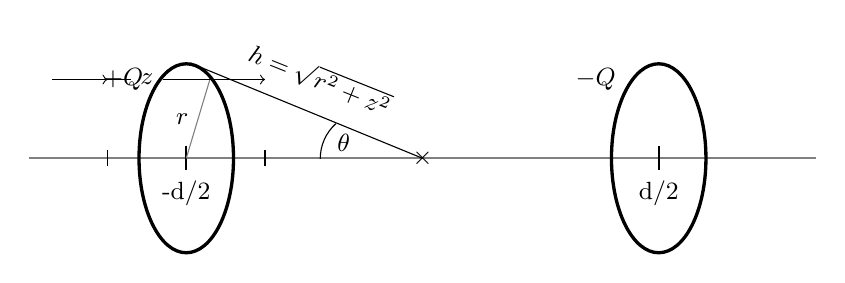
\begin{tikzpicture}
			\tikzmath{\x = 2; \y = -0.9;}
%			-------|--------|------
			\draw [gray, thick](0,0)--(10,0);
			\draw [thick] (2,-0.15)--(2,0.15) node [below, pos=0] {\small -d/2};
			\draw [thick] (8,-0.15)--(8,0.15) node [below, pos=0] {\small d/2};
			\node (c) at (5,0) {\small \( \times \)};
%			figures
			\draw [gray] (2,0)--(2.3,1) node [black, left, pos=0.5] {\small \( r \)};
			\draw (2.05,1.21)--(5,0);
			\node [rotate=-21.8] at (3.7,1) {\small \(h = \sqrt{r^2+z^2} \)};
			\draw (3.9, 0.44) arc (132:180:0.6);
			\node at (4, 0.2) {\small \( \theta \)};
			\draw [very thick] (2,0) ellipse (0.6 and 1.2);
			\node at (1.2,1) {\small \( +Q \)};
			\draw [very thick] (8,0) ellipse (0.6 and 1.2);
			\node at (7.2,1) {\small \( -Q \)};
%			<--- z ---->
			\draw (\x,\y-0.1)--(\x,\y+0.1);
			\draw (\x+3,\y-0.1)--(\x+3,\y+0.1);
			\node at (\x+1.5,\y) {\small{$ z $}};
			\draw [to-] (\x,\y) -- (\x+0.3,\y);
			\draw (\x+0.5,\y) -- (\x+1.3,\y);
			\draw [-to] (\x+1.7,\y) -- (\x+3,\y);
		\end{tikzpicture}\\[2ex]
		Due to the symmetric nature of this problem we can neglect vertical components of forces
		\end{center}	
		\begin{flalign*}
			\mathrm{d}E_1(z) &= k \tfrac{\mathrm{d}Q}{h^2} \cos(\theta) = k \tfrac{\lambda \mathrm{d}r}{r^2 + z^2} \tfrac{z}{\sqrt{r^2 + z^2}} = k \tfrac{\lambda rz}{(r^2 + z^2)^{3/2}} \mathrm{d}\varphi &&\\
			E_1(z) &= \int\ \mathrm{d}E_1 = k \tfrac{\lambda rz}{(r^2 + z^2)^{3/2}} \int\limits_{0}^{2\pi}\ \mathrm{d}\varphi = k \tfrac{\lambda2\pi rz}{(r^2 + z^2)^{3/2}}
			= k \tfrac{Qz}{(r^2 + z^2)^{3/2}} &&\\
			E_2(z) &= -E_1(z-d) = -k \tfrac{Q(z-d)}{(r^2 + (z-d)^2)^{3/2}} &&\\
			E_{ges}(z) &=  E_1 + E_2 = k \tfrac{Qz}{(r^2 + z^2)^{3/2}} -k \tfrac{Q(z-d)}{(r^2 + (z-d)^2)^{3/2}} &&\\
			&= \dl{kQ\left( \tfrac{z+\tfrac{d}{2}}{\left(r^2 + \left(z+\tfrac{d}{2}\right)^2\right)^{3/2}} + \tfrac{\tfrac{d}{2}-z}{\left(r^2 + \left(z-\tfrac{d}{2}\right)^2\right)^{3/2}}\right)} &&
		\end{flalign*}	
		\tcbline
		\item \(  \)
			\( \int\limits_{-d/2}^{d/2}\ qE(z)\ \mathrm{d}z = kQq\left( \int\limits_{-d/2}^{d/2}\ \tfrac{z+\tfrac{d}{2}}{\left(r^2 + \left(z+\tfrac{d}{2}\right)^2\right)^{3/2}}\ \mathrm{d}z + \int\limits_{-d/2}^{d/2}\ \tfrac{\tfrac{d}{2}-z}{\left(r^2 + \left(z-\tfrac{d}{2}\right)^2\right)^{3/2}}\ \mathrm{d}z\right) \\ \)
		\begin{flalign*}
			&= \tfrac{kQq}{2} \left( \int\limits_{r^2}^{r^2+d^2}\ \tfrac{1}{u^{3/2}}\ \mathrm{d}u\ - \int\limits_{r^2-d^2}^{r^2}\ \tfrac{1}{v^{3/2}}\ \mathrm{d}v\right) &&\\
			&= \dl{2kQq \left( \tfrac{1}{r} - \tfrac{1}{\sqrt{r^2+d^2}} \right)} &&
		\end{flalign*}
		\hfill
		\begin{minipage}[t]{0.3\textwidth}
			\vspace{-3.2cm}
			\boxed{
				\begin{aligned}
					u &= r^2 + \left(z + \tfrac{d}{2}\right)^2\\
					\mathrm{d}u &= 2\left(z + \tfrac{d}{2}\right) \mathrm{d}z \\
					v &= r^2 + \left(z - \tfrac{d}{2}\right)^2\\
					\mathrm{d}v &= 2\left(z - \tfrac{d}{2}\right) \mathrm{d}z
				\end{aligned}
			}
		\end{minipage}\\
		\( qE(z) \) represents a force, which in turn gives the amount of work done when integrated over a distance
		\tcbline
		\item \( r = 0.1 \unit{m};\quad d = 0.5 \unit{m};\quad Q = 10^{-6} \unit{C};\quad q = 1.6 * 10^{19} \unit{C};\quad m = 200.592 u \)
		\begin{flalign*}
			W = 2kQq \left( \tfrac{1}{r} - \tfrac{1}{\sqrt{r^2+d^2}} \right) &= \dl{2.3 * 10^{24} \unit{J}} &&
		\end{flalign*}
		\begin{flalign*}
			W &= \tfrac{1}{2} mv^2  &&\\
			v &= \sqrt{\tfrac{2W}{m}} = \dl{3.73 * 10^{24} \unit{\v}} &&
		\end{flalign*}
	\end{enumerate}
\end{mybox}
E6J563C-T5OALEK-AEB6DRY-Q4IP4YP-XVCS2VI-BONPB6R-SHHEMJY-V7465QP


\end{document}